\documentclass[a4paper]{article}
\usepackage[T1]{fontenc}
\usepackage[utf8x]{inputenc}
\usepackage[italian]{babel}

\usepackage{graphicx}
\usepackage{amsmath}
\usepackage{amsthm}
\usepackage{amssymb}
\usepackage{subfigure}
\usepackage{mathtools}
\usepackage{esint}
\usepackage{float}
 \usepackage{import}
\usepackage{xcolor}
\usepackage{geometry}
\geometry{a4paper, top=2cm, bottom=2cm, left=2.5cm, right=2.5cm,  heightrounded, bindingoffset=5mm}

% Quanto segue serve per inserire l'elenco di equazioni
\usepackage[subfigure]{tocloft}
 \newcommand{\listequationsname}{Elenco delle equazioni}
\newlistof{myequations}{equ}{\listequationsname}
\newcommand{\myequations}[1]{%
	\addcontentsline{equ}{myequations}{\protect\numberline{\theequation}#1}\par}
% aggiungere per ogni etichetta oltre \label anche \myequations{NOME}

\usepackage{makeidx} %serve per fare l'indice analitico
% compilare il documento principale
% viene generato un file nome_file.idx
% aprire il file e andare su Strumenti -> Comandi -> \makeindex
% compilare nuovamente il documento iniziale
\makeindex
% aggiungere gli elementi con \index{NOME}
% \index{Voce ! Voce secondaria}

\renewcommand{\thesubsubsection}{}
%rimuove la numerazione dalle sotto-sotto sezione

\title{Formulario fisica tecnica}
\author{}
\date{October 2021}

\begin{document}

\newpage
\maketitle
\newpage
\tableofcontents
\newpage	

\newpage 

Novità rispetto al programma;

Al posto degli esercizi sulla trasmissione del calore verranno raccontate alcune esperienze.
Orale: tre domande di teoria (termodinamica, termofluidodinamica, termocinetica o trasporto di massa) Scritto: due esercitazioni, una sulle miscele aria-vapore (studio del benessere ambientale, saper regolare ambienti in ambienti clinici), cicli frigoriferi, terza domanda semi teorica (raccontare una delle esercitazioni citate sopra). 
Esercitazioni sulla criochirurgia, sulla termoregolazione del corpo umano, sul trasporto di massa in aorta aneurismatica, sul trasporto di massa nel circolo di Willis e sull’acustica ovvero rumore provocato dalle valvole stenotiche. Non ci sono esercizi sulla trasmissione del calore e termofluidodinamica.
Testo: Problematiche di fisica tecnica in ingegneria medica (9 capitoli, da Texmat). Risultati di lavori fatti da colleghi o in tesi di dottorato o nella tesi magistrale ecc.
Lezione interrotta causa problemi di connessione. Appello straordinario; chiedere alla segreteria Scritto e orale nello stesso appello.

\newpage 


\section{Termodinamica}
	 \index{Termodinamica}
\subsection{Introduzione}
	
COMPLETA DA pg 10 


La prima cosa che bisogna fare nella termodinamica classica è definire l’oggetto del nostro studio, cioè l’insieme dei corpi che vogliamo studiare e che chiameremo sistema termodinamico (insieme degli oggetti che vogliamo studiare), si decide quale sistema termodinamico si vuole studiare, ad esempio l’aria nella stanza.
Nel momento in cui decidiamo il sistema, decidiamo anche il contorno fisico del nostro sistema termodinamico S scelto arbitrariamente; quello che c’è all’interno del nostro sistema è l’oggetto del nostro studio, tutto il resto è l’esterno E, mentre S è all’interno del contorno fisico.
Sistema termodinamico   oggetto del nostro studio.
Vogliamo relazionare il sistema termodinamico, cioè quello che c’è all’interno, con l’esterno e in particolare ci interessa la relazione, ovvero le interazioni tra l’interno e l’esterno, cioè ci interessa quello che succede NEL sistema.

COMPLETA 
 \index{Lavoro}
Definizione fisica del \textbf{lavoro}: si parte dal sistema cilindro-pistone \begin{equation}
	l_i=\int_1^2 p_idv
\end{equation}
\label{lavoro}
\myequations{Lavoro}

\textbf{Convenzione termodinamica}: lavoro positivo se fatto dal sistema verso l'esterno.

\textbf{Convenzione termodinamica}: calore positivo se assorbito dal sistema (convezione opposta al lavoro).
\textbf{Temperatura}:



\subsection{Misure}

Grande intensive --> minuscole
Grandezze intensive --> maiuscole

Misura della pressione 

Il barometro misura la pressione assoluta $p_A=\rho g h$

Manometro differenziale: dislivello => differenza di pressione. Bilancio delle forze : $ \rho S+\rho S\Delta z g=p_AS+\rho_m S\Delta z g$
 
Allora si ottiene che la pressione del fluido in esame rispetto la pressione atmosferica è $\rho -\rho_A=\rho_m \Delta zg$ 

\subsection{Frigoriferi ad effetto termoelettrico}


Permettono di misurare la temperatura. 

\textbf{Effetto Seebeck}

COMPLETA

\textbf{Effetto Peltier} completa


\textbf{Effetto Thompson} 
Corrente in un conduttore metallico $\Longrightarrow$ differenza di temperatura. La quantità di calore che viene scambiata con l’esterno è in valore
assoluto proporzionale alla corrente, alla differenza di temperatura e ad un coefficiente che è chiamato coefficiente di Thomson.
$$\left|d \dot{Q}_{T}\right|=|\tau I d T|=\left|\tau I \frac{d T}{d x} d x\right|$$ 

\subsection{Principio zero della termodinamica}

\textbf{Principio zero della termodinamica} o di Fowler. Presi due corpi A in equilibrio con C tramite una parete conduttrice. E il corpo B in equilibrio con lo stesso C. Allora, essendo entrambi in equilibrio con C, saranno A in equilibrio con B. $Longrightarrow$ Possiamo usare C come termoscopio, per misurare se due corpi sono in equilibrio termico. 

\textbf{calore}
È l’interazione tra il sistema termodinamico e l’esterno, che avviene a causa di una differenza di temperatura, attraverso il contorno (tanto all’interno c’è equilibrio e non mi interessa). Questa definizione è generale, c'è anche quella operativa. 

\subsection{Primo principio della termodinamica}
 \index{Primo principio}
Il primo principio della termodinamica stabilisce che il lavoro scambiato in una trasformazione termodinamica {\color{red}{ciclica}} in un sistema {\color{red}{chiuso}} è uguale al calore totale scambiato: 
\begin{equation}
	L=Q
\end{equation}		
\label{primoprincipio}
\myequations{Primo principio della termodinamica}
Ricorda Esperienza di Joule e il fatto che lavoro e calore sono sono negativi (lavoro assorbito e calore ceduto) $-|L|=-|Q|$

Generalizzando vale l'uguaglianza integrale e quindi $dQ-dL=dE$ nota come \textbf{energia totale} e si tratta di una funzione di stato infatti $\oint dE=0$.

L'energia totale dipende da variabili interne e variabili esterne. $E=E_{interne}+E_{esterne}$
Tra le variabili esterne troviamo:
\begin{itemize}
	\item velocità del baricentro
	\item quota del baricentro
\end{itemize}
Allora $\Delta E_e=\Delta E_c+\Delta E_p$ (energia cinetica e potenziale).

Tra le variabili interne troviamo:
\begin{itemize}
	\item variabili termodinamiche (pressione, volume specifico, temperatura)
	\item componenti elettrochimiche (reazioni chimiche, fenomeni elettrici o termoelettrici)
\end{itemize}
Allora $\Delta E_i=\Delta u+\Delta u_x$ (energia interna termodinamica e energia interna di origine elettrochimica).

\textbf{Primo principio della termodinamica per un sistema chiuso che compie trasformazioni aperte}: 
 \index{Primo principio! trasf aperte in un sistema chiuso}
\begin{equation}
	Q-L=\Delta u+\Delta E_c +\Delta E_p 
\end{equation}
\label{1principio}
\myequations{Primo principio}

In termini differenziali:
\begin{equation}
	dq-dl=du+du_x+{dw^2\over 2}+g dz 
\end{equation}
\label{1principiodiff}
\myequations{Primo principio in termini differenziali}

\begin{figure}[h!]
	\begin{center}
		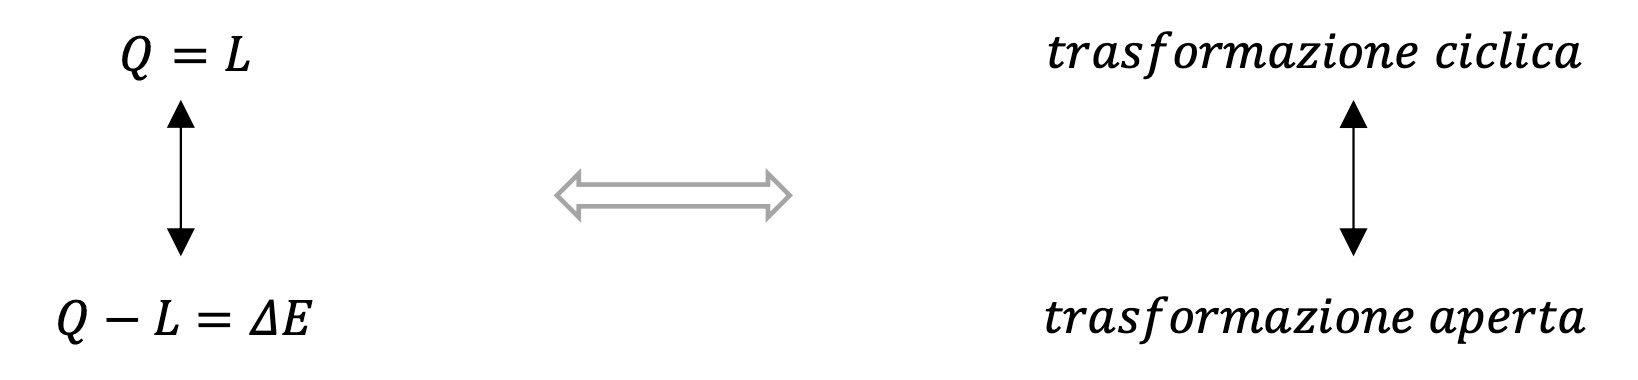
\includegraphics[width=0.6\columnwidth]{generalizprincipio.jpg}
	\end{center}
\end{figure}

\subsection{Sistemi aperti}
Lavoriamo in ipotesi di regime stazionario, in cui vale il bilancio di massa.
$M_t=M_{t+\Delta t}$
\begin{figure}[h!]
	\begin{center}
%		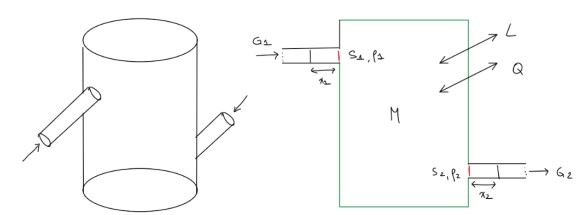
\includegraphics[width=0.6\columnwidth]{sistemaaperto.jpg}
		 \input{sistemaperto.pdf_tex}
	\end{center}
\end{figure}


\textbf{bilancio di energia} $q-l_f-p_2v_2+p_1v_1=\Delta u + \frac{\Delta w^2}{2}+g\Delta z$

Dall'equazione del bilancio dell'energia entra in gioco una nuova grandezza funzione di stato: \textbf{Entalpia}: $h=u+pv$

\begin{equation}
	q-l_f=\Delta h +\Delta e_c + \Delta e_p
\end{equation}
Si definisce Entalpia come il calore scambiato in un sistema aperto dove non è presente lavoro e non ci sono variazioni di energia cinetica e di energia potenziale. $dq=dh$


\subsection{Calore}
\index{Calore}
\textbf{Definizione operativa}: il calore si misura come il lavoro scambiato da un sistema in un'esperienza di Joule. Ovvero un sistema chiuso che compie una trasformazione ciclica. 

\subsection{Secondo principio della termodinamica}
 \index{Secondo principio}
\textbf{Fromulazione di Plank}:
E' impossibile che l'unico risultato di una cessione di calore ad un sistema chiuso che compie trasformazioni cicliche sia la produzione di calore.

\textbf{Fromulazione di Clausius}:
E' impossibile che per un sistema chiuso che compie trasformazioni cicliche l'unico risultato sia la sottrazione di calore da una sorgente inferiore e la cessione di calore ad una sorgente superiore senza alcun effetto compensatorio.

\begin{figure}[H]
	\begin{center}
		\caption{Macchina di Newcomen}
		%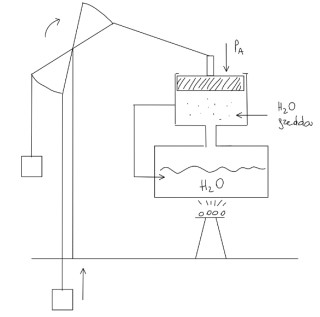
\includegraphics[width=0.4\columnwidth]{macchinaNewcomen.jpg}
				 \input{newcommen.pdf_tex}
	\end{center}
\end{figure}

Definiamo il rendimento come il rapporto tra ciò che si ottiene e ciò che si spende.
Questo meccanismo venne migliorato dalla macchina di Watt;

\begin{figure}[H]
	\begin{center}
		\caption{Macchina di Watt}
		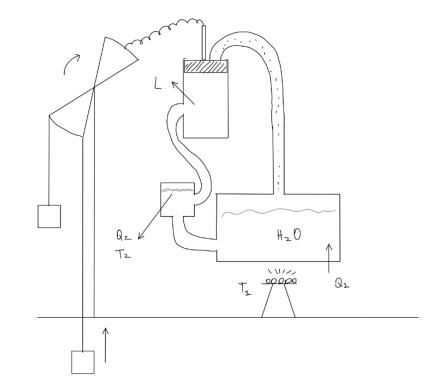
\includegraphics[width=0.6\columnwidth]{macchinadiWatt.jpg}
	\end{center}
\end{figure}

Distinguiamo il calore $Q_1$ che è il calore ceduto dal braciere al sistema termodinamico, il lavoro $L$ come il lavoro positivo esercitato dal sistema verso l'esterno e il calore $Q_2$ come il calore sottratto al sistema per ricondensare il vapore.

Per un sistema termodinamico chiuso che produce lavoro positivo grazie a scambi di calore il limite superiore del rendimento è il rendimento formulato da Carnot: $\eta_{max}=1-\frac{T_2}{T_1}$

\begin{figure}[H]
	\begin{center}
		\caption{Macchina motrice termica}
		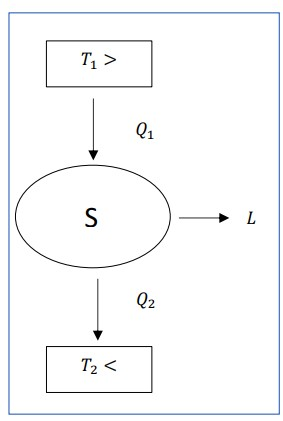
\includegraphics[width=0.2\columnwidth]{sistema.jpg}
	\end{center}
\end{figure}

Carnot fece una similitudine tra il mulino d'acqua e la macchina di Watt;
\begin{itemize}
	\item il lavoro L è lo stesso che produce in entrambi i casi una rotazione
	\item la quota coincide con la temperatura
	\item la portata coincide con il calore
\end{itemize}

il parallelismo errato era quello tra il calore e la portata perchè portava a scrivere $l=Q_1-Q_2=0$
Ma sappiamo che per produrre lavoro positivo la macchina di Watt deve avere $Q_1>Q_2$

Nei sistemi chiusi non si può invertire il segno del calore e del lavoro $\longrightarrow $ fenomeni sono \textbf{irreversibili}

\subsubsection{equivalenza dei principi}
 \index{Secondo principio! equivalenza}

\textbf{nego Plank}

\begin{figure}[H]
	\begin{center}
		\subfigure[Nego Plank]{
		\includegraphics[width=0.25\columnwidth]{Plank.jpg}}
		\subfigure[Nego Celsius]{
		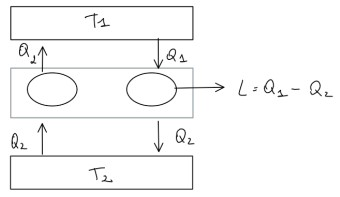
\includegraphics[width=0.4\columnwidth]{Clausius.jpg}}
	\end{center}
\end{figure}

\subsection{Equazioni del secondo principio}
 \index{Secondo principio! equazioni}
\begin{equation}
	\oint \frac{dQ}{T} \le 0
\end{equation}
Questa viene chiamata \textbf{Disuguaglianza di Clausius}; dove T è la temperatura alla quale si scambia calore $dQ$. La disuguaglianza è:
\begin{itemize}
	\item $=0$ per trasformazioni reversibili
	\item $<$ per trasformazioni irreversibili
\end{itemize}

La disuguaglianza di Clausius cambiata di segno è la \textbf{Traccia termodinamica}

\textbf{ciclo diretto}
$\frac{Q_1}{T_1} - \frac{Q_2}{T_2} \le 0 \longrightarrow \frac{Q_{ass}}{T_{ass}} \le \frac{Q_{ced}}{T_[ced]}$

\textbf{ciclo inverso}
$-\frac{Q_1}{T_1} + \frac{Q_2}{T_2} \le 0 \longrightarrow \frac{Q_{ass}}{T_{ass}} \le \frac{Q_{ced}}{T_[ced]}$

Consideriamo la macchina negata della formulazione di Plank e verifichiamo che la disuguaglianza di Clausius sia negata; poichè il calore assorbito è positivo la disuguaglianza di Clausius risulta negata.

\subsection{Entropia}
\index{Entropia}
per una trasformazione reversibile $\oint \frac{dQ}{T}=0$
allora la grandezza $\frac{dQ}{T}=ds$: \textbf{Entropia}

se la trasformazione è irreversibile $\oint\frac{dQ}{T} \le 0$ e quindi possiamo scrivere:
$\frac{dQ}{T}=ds-ds_s$

\textbf{definizione operativa di entropia}
$\Delta s = s_2-s_1=\int_1^2\frac{dq}{T}$

Essendo una funzione di stato è uguale se calcolata lungo trasformazioni reversibili e irreversibili.

\subsubsection{energia interna in funzione dell'entropia}
$dq-dl=du+de_c+de_p$
$du=dq-dl-de_c-de_p$  sappiamo che $dq=Tds$ e $dl=pdv$
\begin{equation}
	du=Tds-pdv
\end{equation}

\subsubsection{entalpia in funzione dell'entropia}
abbiamo definito $h=u+pv$, il differenziale è:
$dh=du+pdv+vdp$
dove $du=Tds-pdv$ quindi:

\begin{equation}
	dh=Tds+vdp
\end{equation}

\subsubsection{teorema dell'aumento di Entropia}
sistema termodinamico isolato con l'esterno, $dq=0$, allora $ds=ds_s$, quindi quando abbiamo trasformazioni irreversibili  il $ds_s$ va ad aumentare l'entropia. 
$ds_s \longrightarrow$ termine di produzione entropica

\subsubsection{sorgenti di produzione entropica}
\begin{itemize}
	\item sorgenti entropiche di prima specie: cause di irreversibilità di prima specie quali differenza di pressione, di temperatura e attriti.
	\item sorgenti entropiche di seconda specie: irreversibilità di prima specie dovute a fenomeni elettrochimici
\end{itemize}

\begin{equation}
	ds_s=ds_{sI}(\Delta p, \Delta T, attriti)+ds_{sII}(x_i,l_{el})
\end{equation}

$dS=dQ\left(\frac{1}{T_2}-\frac{1}{T_1}\right)=dS_{sI}(\Delta T)>0$

$ds_{sI}=(\Delta p)=-\frac{vdp}{T}$








\newpage
\section{Tesine}

\newpage
\section{Indici}
\newpage
\listoffigures
\addcontentsline{toc}{subsection}{\listfigurename}

\newpage
\listoftables
\addcontentsline{toc}{subsection}{\listtablename}
\newpage
\listofmyequations
\addcontentsline{toc}{subsection}{\listequationsname}
\newpage
\addcontentsline{toc}{subsection}{Indice analitico}
\printindex
\newpage








\end{document}